Give a set of real numbers $\Omega$ with cardinality $N$ and allowed $K$ level quantization. Without the loss of generality, we assume that all real numbers in $\Omega$ is in $[0, 1]$. The goal is to decide the optimal $K$ quantization levels $\{p_1, p_2, \cdots, p_{K-1}\}$ for this set to minimize the mean variance
\begin{align}
\nonumber \min_{p_1, \cdots, p_{K-1}}\quad & \mathcal{MV}(p_1,\cdots, p_{K-1}) := {1\over N}\sum_{x\in \Omega} \sum_{k=1}^K {\bf 1}_k(x)V_k(x)\\
\text{s.t.}\quad & 0\leq p_1\leq p_2 \leq \cdots \leq p_{K-1} \leq 1.
\label{eq:opt_Q}
\end{align}
where ${\bf 1}_k(x)$ is the indicator function
\[
{\bf 1}_k(x) = 
\begin{cases}
1 & \text{if}~x\in (p_{k-1}, p_k] \\
0 & \text{o.w.}
\end{cases}
\]
with $p_0=0$ and $p_K=1$, and the $V_k(x)$ is the variance function 
\begin{align}
V_k(x) = (x-p_{k-1})(p_k - x), \label{eq:var}
\end{align}
which is the variance of Bernoulli distribution with probability $p_k-x$ taking value $p_{k-1}$ and probability $x-p_{k-1}$ taking value $p_k$. ${\bf 1}_k(x)V_k(x)$ is the variance if $x$ falls into the interval $(p_{k-1}, p_k]$. 

\paragraph*{Discretization}

This problem is hard to solve directly due to the non-convexity \textcolor{red}{and non-smoothness}. We discretize the range $[0,1]$ into $M$ intervals, that is, $[0,d_1), [d_1, d_2), \cdots, [d_{M-1}, 1]$ with $0< d_1<d_2<\cdots < d_{M-1}<1$. All $p_k$'s are restricted to values in $\{d_1, d_2, \cdots, d_{M-1}\}$ while satisfy the monotonicity. 

\begin{theorem} \label{thm:optQ}
Let the maximal number of points in each interval and the maximal interval length defined by $\{d_m\}_{m=1}^{M-1}$ be bounded by $a/M$ and $bN/M$ respectively. Let $\{p^*_k\}_{k=1}^{K-1}$ and $\{\hat{p}^*_k\}_{k=1}^{K-1}$ be the optimal quantization to \eqref{eq:opt_Q} and the approximate solution using discretization technique introduced above. Let $cM/K$ be the upper bound of the number of small intervals (defined by $\{d_m\}_{m=1}^{M-1}$) crossed by any interval defined by $\{p^*_k\}_{k=1}^{K-1}$. Then we have the discretization error bounded by
\[
 \mathcal{MV}(\hat{p}^*_1,\cdots, \hat{p}^*_{K-1}) -  \mathcal{MV}(p^*_1,\cdots, p^*_{K-1}) \leq {a^2b K \over 4 M^3} + {a^2bc^2 \over MK}.
\]
\end{theorem}
\textcolor{red}{Note that if the numbers of points falling into all intervals defined by $\{d_m\}_{m=1}^{M-1}$ are equal, then constant $a$ is $1$. So $a$ roughly measures the uniformness of the data distribution w.r.t. small intervals. If all intervals defined by $\{d_m\}_{m=1}^{M-1}$ have the equal length, then $b$ is equal to $1$. So $b$ roughly measures the distortion from equal intervals w.r.t. $\{d_m\}_{m=1}^{M-1}$. Similarly, $c$ roughly measures the distortion from equal intervals w.r.t. $\{p^*_k\}_{k=1}^{K-1}$, since $c=1$ means that all intervals defined on $\{p^*_k\}_{k=1}^{K-1}$ roughly cross the same number of small intervals defined by $\{d_m\}_{m=1}^{M-1}$. Theorem~\ref{thm:optQ} suggests that the mean variance using the discrete variance-optimal quantization will converge to the optimal with the rate $O(1/KM)$.}

\paragraph*{Dynamic Programming.}

By introducing this discretization, the following will introduce how to find the optimal solution over the discrete constraint using dynamic programing.  

Define $T(k, m)$ be the optimal total variance for points in $[0, d_m]$ with $k$ quantization levels. Our goal is to calculate $T(K, M)$. This problem can be solved by dynamic programing using the following recursion
\[
T(k, m) = \min_{j\in \{k-1, k, \cdots, m-1\}} T(k-1,j) + V(j,m)
\]
where $V(j,m)$ denotes the total variance of points falling into the interval $[d_j, d_m]$. The optimal value for $p_{K-1}^*$ is $ d_{j^*_{K-1}}$ with $j^*_{K-1}$ equal to
\[
j^*_{K-1} = \argmin_{j\in \{K-1, k, \cdots, M-1\}} T(K-1,j) + V(j,M),
\]
and the rest can be retrieved by 
\begin{align*}
j^*_{k-1} = \argmin_{j\in \{k-1, k, \cdots, j^*_k-1\}} T(k-1, j) + V(j, j^*_k) \\
\text{for all}~k=2, \cdots, K-2
\end{align*}

The complexity of calculating matrix $V(\cdot, \cdot)$ is $O(M^2 + N)$ and the complexity of calculating matrix $T(\cdot, \cdot)$ is $O(KM^2)$. The total memory cost is $O(KM + M^2)$. Note that to solve this optimal quantization, we only need to scan all $N$ numbers once.

Figure~\ref{fig:optimalquantization} shows that for such data distribution, after running our dynamic programming algorithm, 
we get optimal quantization levels.
\begin{figure}[h]
\centering    
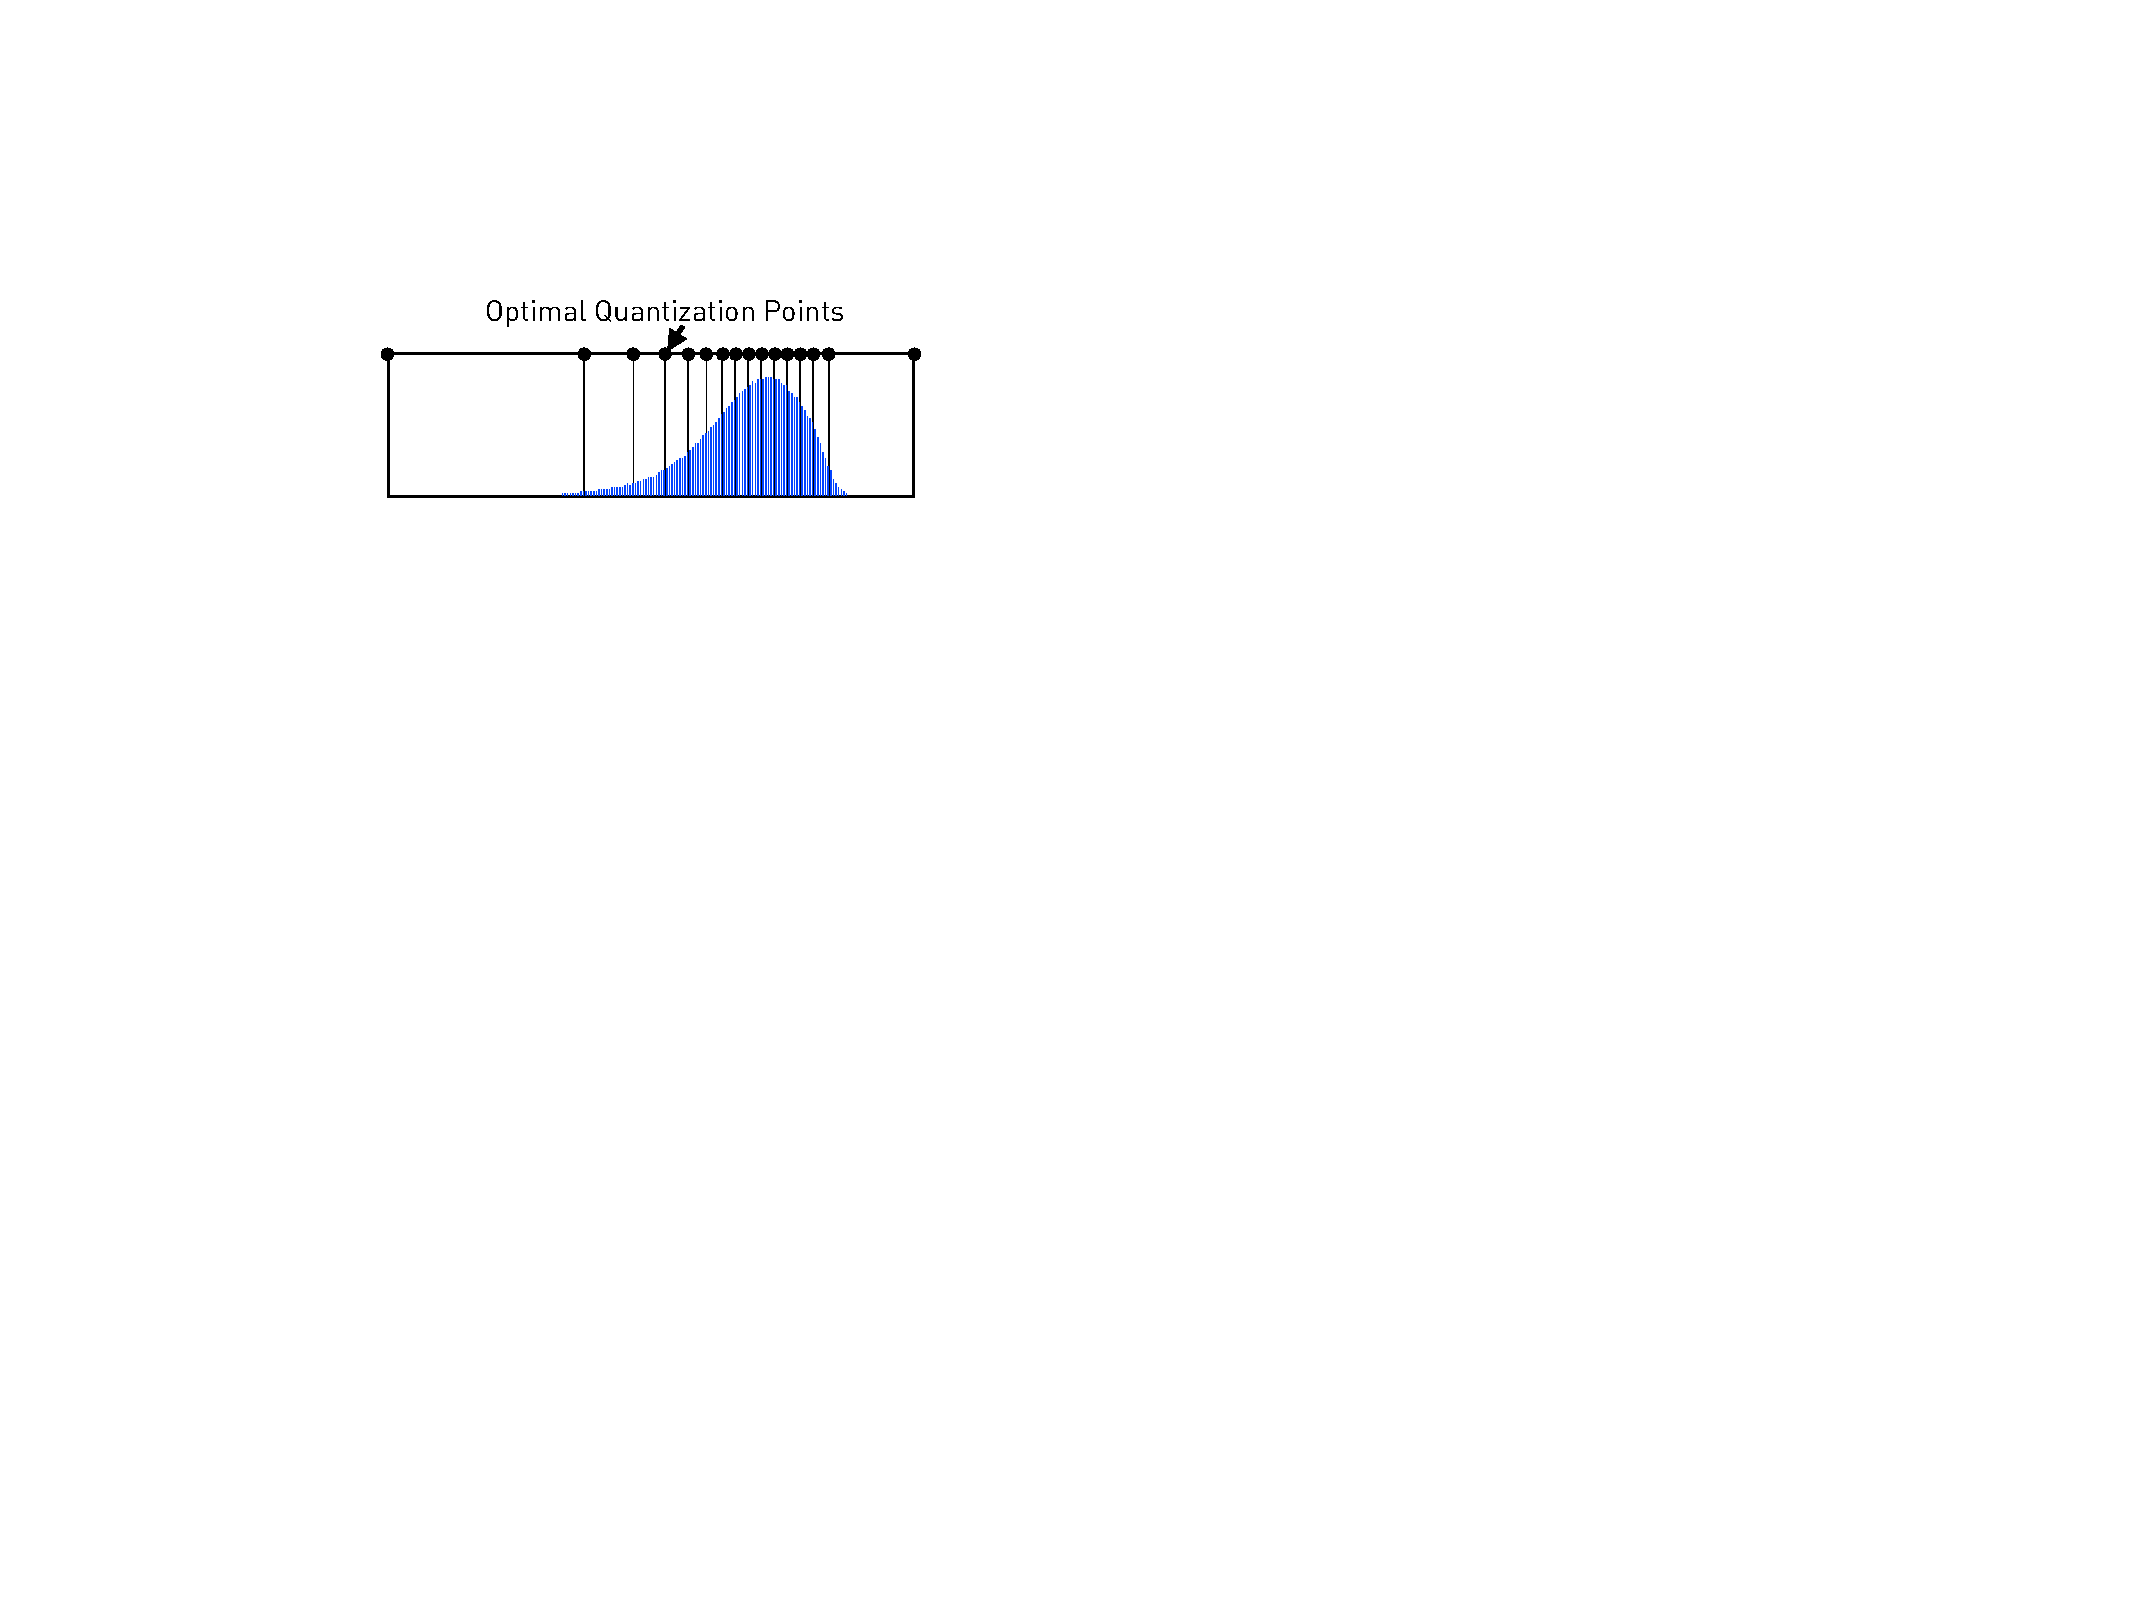
\includegraphics[width=\columnwidth]{micro-experiments/dp-level} 
\caption{An example of using DP to decide optimal quantization levels(16 levels).}
\label{fig:optimalquantization}
\end{figure} 



\iffalse
\begin{proof}
Let $p^*_0$ be $0$ and $p^*_K=1$.We quantitize $\{p^*_k\}_{k=1}^{K-1}$ one element by one element, while monitor the changing of the total variance $N \times \mathcal{MV(\cdot)}$. We first quantize $p^*_1$ to the closest value (denoted it by $Q(p^*_1)$) in $\{d_m\}_{m=1}^{M-1} \cup \{p^*_0,p^*_K\}$ under the monotonicity constraint, that is, $p^*_0\leq Q(p^*_1) \leq p^*_2$. Here, one important observation is $|p^*_{1} - Q(p^*_1)|\leq a/M$. Consider the total variance of this new solution $Q(p^*_1), p^*_2, \cdots, p^*_{K-1}$. The variance of points falling into the range $[p^*_2, 1]$ does not change at all. Without the loss of generality, assume $p^*_{1} \geq Q(p^*_1)$.

Next we consider points falling into the following three sets $C_1 = [p^*_0, Q(p^*_1)]$, $C_2 = [Q(p^*_1), p^*_1]$, and $C_3 = [p^*_1, p^*_2]$. The variance of points of falling into $C_1$ gets reduced from the form of variance in \eqref{eq:var}. Next we only need to check the variance change for points in $C_2$ and $C_3$. Consider $C_2$ first. The variance for point $x$ in $C_2$ is
\[
(x-Q(p^*_1))(p^*_1 - x) \leq {a^2 \over 4 M^2}. 
\]  
Thus, the change of variance for points in $C_2$ would be bounded by ${a^2 \over 4 M^2}$. Then consider $C_3$. The change of variance for point $x$ in $C_3$ is
\begin{align*}
& (x-Q(p^*_1))(p^*_2 - x) - (x-p^*_1) (p^*_2 - x) 
\\
= & (p^*_1 - Q(p^*_1)) (p^*_2 - x)
\\
\leq & {a\over M}(p^*_2 - x)
\end{align*}
Therefore, the change of total variance from $\{p^*_1, p^*_2, \cdots, p^*_{K-1}\}$ to $\{Q(p^*_1), p^*_2, \cdots, p^*_{K-1}\}$ is bounded by 
\begin{align}
\nonumber
& \sum_{x\in C_2} {a^2 \over 4M^2} + \sum_{x \in C_3} {a\over M}(p^*_2 - x)
\\
\nonumber
\leq & {Nb \over M} {a^2 \over 4M^2} + {a\over M}{Nb \over M} \sum_{t=1}^{cM/K}t{a\over M}
\\
\leq &
{a^2b N \over 4 M^3} + {a^2bc^2 N \over MK^2}
\label{eq:bound_1step}
\end{align}
Similarly, we quantitize $p^2_2$ in $\{Q(p^*_1), p^*_2, \cdots, p^*_{K-1}\}$ to get a new solution $\{Q(p^*_1), Q(p^*_2), \cdots, p^*_{K-1}\}$ while maintain the monotonicity. We can establish the same upper bound to \eqref{eq:bound_1step}. Following this idea, we can obtain a quantization solution $\{Q(p^*_1), Q(p^*_2), \cdots, Q(p^*_{K-1})\}$. Therefore, we obtain that 
\begin{align*}
&  \mathcal{MV}(Q(p^*_1), Q(p^*_2), \cdots, Q(p^*_{K-1})) -  \mathcal{MV}({p}^*_1,\cdots, {p}^*_{K-1}) 
 \\
 & \quad \leq {a^2b K \over 4 M^3} + {a^2bc^2 \over MK}.
\end{align*}
Using the fact that $ \mathcal{MV}(p^*_1,\cdots, p^*_{K-1})$ is smaller than $\mathcal{MV}(Q(p^*_1), Q(p^*_2), \cdots, Q(p^*_{K-1}))$ proves the claim.
\end{proof}
\fi















